% Options for packages loaded elsewhere
\PassOptionsToPackage{unicode}{hyperref}
\PassOptionsToPackage{hyphens}{url}
%
\documentclass[
  10pt,
]{article}
\usepackage{amsmath,amssymb}
\usepackage{iftex}
\ifPDFTeX
  \usepackage[T1]{fontenc}
  \usepackage[utf8]{inputenc}
  \usepackage{textcomp} % provide euro and other symbols
\else % if luatex or xetex
  \usepackage{unicode-math} % this also loads fontspec
  \defaultfontfeatures{Scale=MatchLowercase}
  \defaultfontfeatures[\rmfamily]{Ligatures=TeX,Scale=1}
\fi
\usepackage{lmodern}
\ifPDFTeX\else
  % xetex/luatex font selection
  \setmainfont[]{STIX}
  \setmathfont[]{STIX Math}
\fi
% Use upquote if available, for straight quotes in verbatim environments
\IfFileExists{upquote.sty}{\usepackage{upquote}}{}
\IfFileExists{microtype.sty}{% use microtype if available
  \usepackage[]{microtype}
  \UseMicrotypeSet[protrusion]{basicmath} % disable protrusion for tt fonts
}{}
\makeatletter
\@ifundefined{KOMAClassName}{% if non-KOMA class
  \IfFileExists{parskip.sty}{%
    \usepackage{parskip}
  }{% else
    \setlength{\parindent}{0pt}
    \setlength{\parskip}{6pt plus 2pt minus 1pt}}
}{% if KOMA class
  \KOMAoptions{parskip=half}}
\makeatother
\usepackage{xcolor}
\usepackage[top=0.78in,bottom=0.78in,left=0.86in,right=0.86in]{geometry}
\setlength{\emergencystretch}{3em} % prevent overfull lines
\providecommand{\tightlist}{%
  \setlength{\itemsep}{0pt}\setlength{\parskip}{0pt}}
\setcounter{secnumdepth}{5}
\ifLuaTeX
\usepackage[bidi=basic]{babel}
\else
\usepackage[bidi=default]{babel}
\fi
\babelprovide[main,import]{american}
\ifPDFTeX
\else
\babelfont{rm}[]{STIX}
\fi
% get rid of language-specific shorthands (see #6817):
\let\LanguageShortHands\languageshorthands
\def\languageshorthands#1{}
% Stage 4 journal typography — XeLaTeX / STIX family.
% Restrained typesetting: no colored boxes, no decorative graphics, no oversized headings.
\usepackage{microtype}
\usepackage{booktabs}
\usepackage{graphicx}
\usepackage{tabularx}
\usepackage{threeparttable}
\usepackage{hanging}
\usepackage{array}
\usepackage{caption}
\usepackage{float}
\usepackage{placeins}
\usepackage{needspace}
\usepackage{titlesec}
\usepackage{fancyhdr}
\usepackage{ragged2e}
\usepackage{setspace}
\usepackage{xurl}
\usepackage{seqsplit}
\usepackage{hyperref}
\setstretch{1.11}
\setlength{\parindent}{1.25em}
\setlength{\parskip}{0pt plus 1pt}
\setlength{\emergencystretch}{2em}
\titlespacing*{\section}{0pt}{1.65\baselineskip}{.48\baselineskip}
\titlespacing*{\subsection}{0pt}{1.2\baselineskip}{.38\baselineskip}
\titleformat{\section}{\large\bfseries}{\thesection}{.7em}{}
\titleformat{\subsection}{\normalsize\bfseries}{\thesubsection}{.7em}{}
\titleformat{\subsubsection}{\normalsize\itshape}{\thesubsubsection}{.7em}{}
\captionsetup[table]{font=small,labelfont=bf,labelsep=period,
  justification=raggedright,singlelinecheck=false,skip=5pt}
\captionsetup[figure]{font=small,labelfont=bf,labelsep=period,
  justification=raggedright,singlelinecheck=false,skip=5pt}
\setlength{\textfloatsep}{13pt plus 2pt minus 2pt}
\setlength{\floatsep}{11pt plus 2pt minus 1pt}
\setlength{\intextsep}{11pt plus 2pt minus 1pt}
\setlength{\tabcolsep}{5pt}
\renewcommand{\arraystretch}{1.20}
\pagestyle{fancy}
\fancyhf{}
\fancyhead[R]{\footnotesize\textsc{Redistricting simulation methods}}
\fancyfoot[C]{\footnotesize\thepage}
\renewcommand{\headrulewidth}{0pt}
\setlength{\headheight}{13.5pt}
\urlstyle{same}
\hypersetup{colorlinks=true,linkcolor=black,urlcolor=black,
  citecolor=black,pdfauthor={Research manuscript},pdftitle={When a Random Map Is Not a Neutral Map}}
\AtBeginDocument{\raggedbottom}
\ifLuaTeX
  \usepackage{selnolig}  % disable illegal ligatures
\fi
\IfFileExists{bookmark.sty}{\usepackage{bookmark}}{\usepackage{hyperref}}
\IfFileExists{xurl.sty}{\usepackage{xurl}}{} % add URL line breaks if available
\urlstyle{same}
\hypersetup{
  pdflang={en-US},
  hidelinks,
  pdfcreator={LaTeX via pandoc}}

\author{}
\date{}

\begin{document}

\begin{center}
{\fontsize{17.2}{20}\selectfont\bfseries The Phantom Baseline\par}
\vspace{5pt}
{\fontsize{11.2}{14}\selectfont Geographic Assumptions, Mixing Failures, and Constraint Sensitivity
in Computational Redistricting\par}
\vspace{9pt}
{\footnotesize Research methods and computational sensitivity study \enspace$\cdot$\enspace October 2026\par}
\end{center}
\vspace{5pt}

\begin{abstract}
An ensemble's apparent objectivity depends on how its baseline was constructed. We investigate three independently testable vulnerabilities in computational redistricting—geographic topology, Markov-chain exploration, and constraint dependence—using source-matched Michigan precinct geography and counterfactual presidential-vote overlays. First, a previously used graph-repair procedure selected five artificial edges according to enacted congressional labels; the endpoint polygons were separated by approximately 42–280 km. A district-blind proximity alternative retained reference connectivity with 13 candidate links and a maximum separation of 17.8 km, although the resulting graph is not an independently certified legal adjacency model. Second, multi-chain diagnostics rejected the treatment of tested sampler outputs as converged ensemble draws: one ReCom condition yielded rank-normalized R-hat 1.733 and bulk effective sample size 9.4; a local reversible Metropolis–Hastings configuration yielded R-hat 2.588. Third, we implement a deliberately specified finite-horizon stress test, rather than infer a stationary law from failed convergence. Across 64 separately seeded 800-transition terminal maps, relaxing a composite set of geographic caps increased precinct reassignment by 15.61 percentage points and reduced mean Democratic seats by 0.406 and mean efficiency gap by 0.03278. The tighter-minus-relaxed efficiency-gap contrast had a paired-bootstrap 95\% interval of [+0.00975, +0.05631]. We use these results to define an operational baseline reliability protocol: source-grounded topology, target-specific exploration evidence, and explicit assumption-sensitivity checks. The experiments identify how a reproducible computational baseline can depend materially on modeling decisions; they do not claim to establish the distribution of all lawful Michigan maps.

\end{abstract}

\noindent\textbf{Keywords.} redistricting; gerrymandering; Markov chain
Monte Carlo; ReCom; graph topology; computational reproducibility;
sampling convergence; geographic sensitivity; Michigan.

\hypertarget{introduction}{%
\section{Introduction}\label{introduction}}

A redistricting ensemble does not become an objective baseline simply
because it contains many maps. What a histogram means depends on the
graph used to define districts, the rules that determine admissibility,
the transition kernel that explores them, and whether the resulting
sample adequately approximates the claimed distribution. These are
substantive modeling decisions. A stable-looking percentile does not
independently establish that its counterfactual alternatives were
neutral or legally plausible.

That distinction matters whenever ensemble rankings are treated as
evidence of representational bias. A statement that an enacted plan is
rare among simulated alternatives implicitly asserts that the simulation
approximates a justified distribution over relevant maps. The apparent
precision of a percentile cannot substitute for establishing this link.
The redistricting literature already contains important work on
recombination methods, simulation validation, and legally attentive
state-level sampling (DeFord, Duchin, and Solomon 2021; McCartan et
al.~2022; Kenny et al.~2023). We do not treat the field's existing
methods as uniformly defective. We examine a concrete pipeline to
identify the vulnerabilities that any claimed baseline should be able to
survive.

The empirical analysis is organized around three failure channels.
Topology: arbitrarily inserted graph edges can determine which
congressional districts count as connected, and conditioning such
repairs on the enacted map can contaminate a purportedly external
baseline. Mixing: a chain may make many proposals or record thousands of
maps without supplying independent information about the intended
stationary law. Constraint selection: altering researcher-specified
fragmentation caps can change the finite-horizon distribution of both
geographic movement and partisan outcomes.

We investigate these channels using pinned 2020 Michigan precinct data.
Original polygon geometry permits the measurement of artificial-edge
separations. Independently seeded multi-chain studies supply
rank-normalized convergence diagnostics. A separate, expressly
finite-horizon experiment produces 64 independently verified terminal
assignments, with 32 seed-indexed runs in each of two composite
constraint regimes. On the same model graph and 2020 presidential-vote
overlay, relaxing those caps increased mean precinct reassignment by
15.61 percentage points while decreasing Democratic seats by 0.406 and
efficiency gap by 0.03278. This signed direction matters: a comparison
of two modeled procedures is not a generic statement that relaxing rules
benefits a particular party.

Our contribution is an executable way to interrogate a baseline, not a
new asymptotic sampling theorem. We turn the case findings into three
auditable gates---independent geographic provenance, target-specific
sampling diagnostics, and a quantitative constraint-perturbation
check---each with records, criteria, and failure consequences. The study
demonstrates why these gates are operationally consequential in one
source-reconciled experiment. Establishing how often published analyses
or expert testimony fail them remains a separate empirical task.

The paper first formalizes the computational baseline and verifies its
sources. It then presents the topology, mixing, and constraint
experiments, followed by a failure-oriented reliability protocol that
researchers can apply before interpreting simulated maps as a neutral
comparison.

\hypertarget{defining-a-computational-baseline}{%
\section{Defining a computational
baseline}\label{defining-a-computational-baseline}}

\hypertarget{geographic-topology-defines-the-state-space}{%
\subsection{Geographic topology defines the state
space}\label{geographic-topology-defines-the-state-space}}

Represent a precinct-level state as an undirected graph \(G=(V,E)\).
Each vertex \(v\) is a geographic unit with population \(p_v\) and
election attributes; an edge asserts adjacency under a defined
geographic rule. A congressional map is an assignment
\(x:V\rightarrow\{1,\ldots,K\}\), where here \(K=13\). For each district
label \(d\), the induced subgraph \(G[x^{-1}(d)]\) should be connected
\emph{under the chosen adjacency definition}. Population equality can be
imposed by

\begin{equation}
\begin{aligned}
P^{\star} &= \frac{1}{K}\sum_{v\in V}p_v, \\
P_d(x) &= \sum_{\{v\in V:\,x(v)=d\}}p_v,\\
\left|\frac{P_d(x)}{P^{\star}}-1\right| &\leq \varepsilon,
\qquad d=1,\ldots,K.
\end{aligned}
\end{equation}

where \(P_d(x)\) is district population, \(P^{\star}\) is the
equal-population ideal and \(\varepsilon\) is the tolerance applied by
the particular experiment.

This formalization immediately exposes a substantive problem: graph
connectivity is not identical to legally acceptable contiguity.
Michigan's Constitution, article IV, section 6(13), explicitly addresses
geographic contiguity and treats islands as contiguous by land to the
county of which they are part. It also establishes a ranked set of
considerations that includes federal law and the Voting Rights Act,
communities of interest, partisan fairness, consideration of
county/city/township boundaries, and reasonable compactness. A model in
which a precinct becomes ``adjacent'' because it is the nearest polygon
across water need not satisfy those rules. Nor do generic cut-edge or
county-split penalties encode them exactly. A computational state space
is therefore a proposed \emph{model of admissibility}, not a legal
determination.

\hypertarget{the-transition-kernel-and-its-target}{%
\subsection{The transition kernel and its
target}\label{the-transition-kernel-and-its-target}}

Even after selecting a graph and feasible set \(S\), an ensemble needs a
probability law \(\pi\) over maps. Uniformity over labeled maps,
uniformity over unlabeled district partitions and a
spanning-tree-weighted distribution are different constructions. They
need not agree on the frequency of a particular partisan score. A
transition kernel \(P(x,y)\) should be assessed relative to that
intended law: stationarity requires \(\pi P=\pi\), while detailed
balance is the stronger sufficient condition
\(\pi(x)P(x,y)=\pi(y)P(y,x)\). An irreducibility and practical-mixing
argument is still needed to say that finite runs approach the intended
law from their starting states.

Ordinary ReCom proposes a new pair of districts by merging adjacent
districts, constructing a spanning tree and splitting it into
population-balanced connected parts (DeFord et al.~2021). Its strong
spatial movement can be useful, but the name ``ReCom'' alone does not
identify a universal stationary distribution, especially when custom
hard rejections alter the implementation. In contrast, Cannon et
al.~(2026) describe a reversible recombination kernel targeting a
distribution weighted by district spanning-tree counts. That theorem
applies under its specified kernel and state-space assumptions; simply
invoking a library routine, adding undocumented geographic restrictions,
or running it for a small number of steps does not establish mixing on
the present Michigan model.

The distinction between \emph{a mathematically known invariant law} and
\emph{empirical exploration of it} underlies this paper. A theoretically
reversible chain can be immobile. An active chain can have an unknown
target. Neither output should automatically be treated as a sample of
legal maps. The literature supplies different mathematical objects
rather than a single algorithmic guarantee: the reversible
spanning-tree-weighted law discussed by Cannon et al.~(2026) is not the
uniform-within-communicating-class law targeted by our separately
implemented local boundary-edge Metropolis--Hastings (MH) kernel.
Failure of the latter to mix cannot falsify the former's reversibility
theorem. It can demonstrate the practical gap between verifying detailed
balance for a specified kernel and obtaining informative finite-budget
samples from that kernel.

\hypertarget{interpretation-of-partisan-scores}{%
\subsection{Interpretation of partisan
scores}\label{interpretation-of-partisan-scores}}

We use Democratic seats under a fixed two-party presidential vote
overlay and the efficiency gap. Following Stephanopoulos and McGhee
(2015), the efficiency gap is the difference between wasted Republican
and Democratic votes, divided by total two-party votes. In the project's
sign convention,

\begin{equation}
\operatorname{EG}(x)
=\frac{W_R(x)-W_D(x)}{V_R(x)+V_D(x)}.
\end{equation}

A positive value indicates more Republican than Democratic wasted votes
under this convention; a negative value indicates the reverse. Wasted
votes consist of votes for the losing party and votes for the winning
party beyond its defined winning threshold. The implemented threshold is
\texttt{floor(total\_two\_party\_votes/2)+1}. Because 2016 precinct
allocations contain fractional votes, that floor operation makes
individual district wasted-vote totals slightly sensitive to floating
summation order. The source audit identified and bounded a
one-vote-level difference in the archived 2016 reference efficiency gap;
the discrepancy is numerically small but should not be concealed as
exact agreement.

An efficiency gap or seat count is not, on its own, evidence of intent,
legal invalidity or discriminatory effect. Even a perfectly computed
score remains conditional on the overlay election, turnout distribution,
districting graph, and law assigned to the alternative maps. In this
study the 2016 and 2020 \emph{presidential} vote fields are applied
counterfactually to the congressional plan adopted in 2021; they are not
observed congressional-election outcomes under that plan.

\hypertarget{source-verification-and-measurement}{%
\section{Source verification and
measurement}\label{source-verification-and-measurement}}

\hypertarget{provenance-and-processed-precinct-graph}{%
\subsection{Provenance and processed precinct
graph}\label{provenance-and-processed-precinct-graph}}

The principal Michigan source is the processed
election/population/precinct dataset published by Ellen Veomett and
collaborators Arbie Hsu and Alusi, using Redistricting Data Hub inputs
and the \texttt{maup} geographic-processing library. Their data
documentation identifies the 2020 Census population layer, VEST
2016/2020 presidential vote allocations and 2021 adopted congressional
district field. The original published JSON graph is pinned by Git blob
\texttt{\seqsplit{a4dfe70818f87b97924781216f3d86a672cfc66a}}; the
matching original precinct polygon ZIP by
\texttt{\seqsplit{07bce18dabbcca9d549e28995a8156fd6978d7db}}. The source
files are governed by the authors' CC BY-NC 4.0 terms together with the
applicable Redistricting Data Hub terms.

The original processed Michigan graph has 4,756 vertices, 12,378 edges,
six connected components and 13 enacted congressional labels. Summed
precinct population is 10,077,331, giving an ideal of 775,179.31 persons
per district. The reference's maximum district deviation from that ideal
is approximately 0.4019\%. Independently inspecting the published
shapefile confirms its coordinate system as EPSG:32616. All 4,756 graph
nodes were reconciled with polygon records on population, enacted label
and county identifiers. This establishes processed-input matching, not a
new recreation of the full upstream Census/VEST block-to-precinct data
join or agreement with official election canvasses.

Under the processed 2020 presidential fields, statewide two-party totals
are 2,804,046 Democratic and 2,649,864 Republican votes. The enacted
reference gives seven Democratic seats and efficiency gap +0.0033332
under the project's arithmetic. The processed 2016 presidential layer
yields six Democratic seats and efficiency gap approximately −0.0387493,
subject to the tiny rounding issue noted above. These reference
calculations were independently reproduced by summing graph-node vote
fields and reconciled against six saved initial-chain rows and 26
district-level election rows.

Provenance must extend from input identity to reported output. The
processed source graph and polygon archive are checked against their
specified Git blob hashes; the regenerated 13-edge KNN3 sensitivity
graph is identified by SHA-256
\texttt{\seqsplit{14355742f58291f4c26267982de07a21037c347f7598a68f032e0d68ea1d542c}}.
The finite-horizon workflow records endpoint assignment hashes and RNG
seeds, independently rescores terminal plans, and produces a derived
data artifact used by the Stage 4 vector-figure pipeline. This reduces
opportunities for undocumented manual substitution between simulation
and visualization. Content digests alone cannot verify the correctness
of the upstream joins, the choice of model, or the interpretation of a
figure; they establish file identity, not inferential validity.

\hypertarget{independent-computational-checks}{%
\subsection{Independent computational
checks}\label{independent-computational-checks}}

Reproducibility was assessed at different levels rather than reduced to
a single ``tests passed'' declaration. Source identities were checked
against exact published byte hashes. Original archived scalar histories
were reanalyzed directly from the checked-in research ZIP rather than
trusting their saved summary tables. Polsby--Popper, convex-hull ratio
and Reock compactness scores were independently recalculated for all 13
reference districts from source-matched polygons; the Reock check used
GEOS/Shapely's minimum-bounding-radius routine rather than the project's
earlier randomized enclosing-circle implementation. At the code level,
new adversarial tests deliberately introduce and reject malformed step
indices, impossible seat counts, invalid population deviations,
nonfinite precinct vote counts and other corrupt inputs. The checks test
how analysis code fails when supplied invalid evidence rather than
merely confirming that a nominally valid analysis completes. Separately,
the finite-horizon experiment independently validates all 64 terminal
assignments, and the longer mixing pilots independently verify their
archived periodic snapshots. These are materially different coverage
claims: the CI suite does not independently rescore every intermediate
state at every MCMC step.

These checks support the numerical and engineering claims made in
subsequent sections. They cannot recover the full precinct assignments
of historical chains that saved only scalar time series. They also do
not verify the upstream raw Census/VEST joins or the legal admissibility
of any sampled map. These omissions are treated as limits of the
evidence, not as features that can be inferred from the consistency of
derived tables.

\hypertarget{pillar-i-topological-vulnerability}{%
\section{Pillar I: Topological
vulnerability}\label{pillar-i-topological-vulnerability}}

\hypertarget{the-hidden-role-of-artificial-adjacency}{%
\subsection{The hidden role of artificial
adjacency}\label{the-hidden-role-of-artificial-adjacency}}

The published Michigan graph contains six disconnected components, a
common difficulty for land-based precinct graphs with island, shoreline
or water-separated pieces. The original project made the graph connected
by repeatedly identifying a disconnected component and a vertex in the
principal component that shared an enacted congressional district label.
It then added an artificial edge between arbitrarily selected vertices
of that common label. The logic was convenient: it made the reference
districts connected without explicitly changing their precinct
assignments. But it encoded the enacted map into the connectivity repair
itself.

When the original published precinct polygons were consulted, the five
artificial edges proved to span roughly 42, 117, 134, 170 and 280
kilometers between their endpoint polygons. They were not chosen to
represent contact, geographic proximity, county-island rules or a
documented transport corridor. An algorithm that subsequently assesses
``contiguity'' on the augmented graph inherits these unsupported
connections. The fact that a reference map passes contiguity in such a
graph therefore offers little independent evidence that the model
reproduces physical or legal geography.

This is not merely a cartographic imperfection. The graph \texttt{E}
determines which precinct reassignment moves are feasible, which
districts count as contiguous and how many cut edges a plan has.
Artificial edges can also change proposal probabilities for
boundary-driven Markov chains. In addition, conditioning the
construction of \texttt{E} on the enacted label \texttt{CD} undermines a
comparison intended to treat the enacted map as an external object
evaluated against alternatives.

Cross-state scope and the local-anomaly hypothesis. The Michigan result
is unusually vivid because its coastline and island geography expose the
distance between graph connectivity and physical geography. Yet the
underlying methodological hazard is not logically confined to states
with complex shorelines. Precinct dual graphs depend on the chosen
rook-versus-queen adjacency convention, the treatment of zero-width
contacts, boundary precision, invalid or overlapping polygons, and the
reconciliation of units from different administrative datasets. Any of
these choices can alter the graph used to enforce district contiguity or
count district-boundary cuts. A landlocked comparison is therefore a
useful way to test whether the \emph{audit problem} persists after
removing Michigan's most obvious geographical explanation. The existing
repository includes a
\href{https://github.com/DjokovicMan22/Gerrymandering-Project/blob/research/stages-1-3-validation/outputs/figures/week1/mo_precinct_dual_graph_overlay.png}{Missouri
precinct dual-graph overlay}, alongside descriptive election and
precinct outputs.

What the Missouri illustration does---and does not---establish. This
overlay documents that a Missouri precinct graph was generated and
visualized, but visual separation between plotted vertices cannot
establish that the underlying graph has disconnected components; nor can
a saved image identify whether any exceptional edges were inserted, were
geographically valid, or depended on enacted district labels. The
original local Missouri inputs were not byte-matched to a published
processed source during the Michigan audit, and no Missouri component
inventory, GIS distance audit, or independent bridge ledger was
completed under the present protocol. Therefore, the Missouri figure is
a cross-state diagnostic lead, not a second-state replication or proof
of nationwide prevalence. A genuine cross-state extension would first
pin the Missouri polygon and graph bytes, enumerate connected components
and disconnected within-district pieces, reconstruct every non-source
adjacency, calculate polygon separations under a documented CRS, and
compare those connections with locally applicable geographic and legal
rules. The generalizable warning is nonetheless exact: an unexplained
synthetic edge changes the model's feasible state space regardless of
which state contains it. Claims that this particular pathology is common
nationally require additional independently audited states.

\begin{figure}[H]
\centering
\includegraphics[width=0.76\linewidth,height=0.56\textheight,keepaspectratio]{../../figures/week1/mo_precinct_dual_graph_overlay.png}
\par\smallskip
{\footnotesize \textbf{Supplementary Figure S1.} Exploratory Missouri precinct dual-graph overlay from prior work. Its source bytes, graph components and inserted adjacency were not independently verified under this audit; the visual does not establish Missouri replication or national prevalence.}
\end{figure}

\hypertarget{geometric-repair-reference-compatibility-and-selection-bias}{%
\subsection{Geometric repair, reference compatibility and selection
bias}\label{geometric-repair-reference-compatibility-and-selection-bias}}

The first replacement joined original graph components using a
minimum-spanning tree based on measured polygon-to-polygon distance,
without consulting district labels when proposing edges. Its total
proposed connection length fell to approximately 19.6 kilometers.
However, the resulting graph still left a four-precinct piece of the
enacted sixth district disconnected. Rather than repair the failure by
adding another enacted-label-conditioned connection, we examined a
predeclared sensitivity grid of \emph{K} nearest external polygon
contacts per original disconnected component, with \emph{K} taking
values 1, 3, 10, 25 and 50.

The smallest tested neighborhood level that simultaneously connected the
statewide graph and allowed all 13 enacted reference districts to be
represented as connected was K=3, yielding 13 distinct inserted edges.
The longest candidate polygon separation was approximately 17.8
kilometers. Under this model graph, the enacted reference has 682 graph
cut edges, versus 681 on the untouched published source graph. Source
graph and generated-graph hashes were checked in independent workflow
runs.

This construction avoids \emph{directly} using partisan returns or
enacted labels to select individual edges. Yet the choice of K=3 was
made \emph{after} testing whether the reference itself remained
representable. The overall modeling decision is thus still partly
reference-conditioned. More importantly, geographic nearness alone does
not certify Michigan's statutory island/county contiguity: some
candidate connections span nonzero gaps between polygons and may cross
water. The resulting KNN3 graph is therefore best described as an
explicit proximity-based sensitivity topology. It is not a legal
replacement for an authoritative adjacency model.

A general principle follows: selecting boundary conventions by how well
they preserve the benchmark plan can introduce a subtle
baseline-selection mechanism even when a local edge-selection routine
never reads election data. An analytically legitimate neutral benchmark
would require an adjacency convention grounded independently in
geography and applicable law \emph{before} assessing the enacted plan.

\hypertarget{an-automated-topology-audit-not-an-automatic-geography-certificate}{%
\subsection{An automated topology audit, not an automatic geography
certificate}\label{an-automated-topology-audit-not-an-automatic-geography-certificate}}

The topology diagnosis was converted into executable checks. The
\texttt{stage3-bridge-audit.yml} workflow retrieves the pinned original
4,756-node graph, verifies its Git blob identity, reconstructs the five
historical \emph{project-added} connections, and reports which endpoints
disagree on source county identifiers. All five historical artificial
bridges cross county identifiers. That is an anomaly requiring
investigation---not proof of unlawful adjacency, since legitimate
county-to-county borders exist. The geometric distance audit, rather
than the county labels alone, exposes why those particular bridges were
unsuitable as independently justified geographic contacts.

The independent component-distance experiment
(\texttt{stage3-geometric-mst-candidates.yml}) constructs a
minimum-spanning tree among the six disconnected source components using
projected polygon distance and without inspecting congressional labels.
Its five candidate separations range from 0 to 14.90 km, totaling
approximately 19.63 km. This distance-minimizing solution nonetheless
fails to preserve contiguity of every enacted reference district under
the resulting candidate model, as recorded by
\texttt{validate\_candidate\_topology.py}. This distinguishes geometric
optimization from reference compatibility: optimizing proximity alone
does not settle the geographic model. The subsequently tested KNN3
procedure preserved the 13 enacted reference districts with 13 added
proximity links; its maximum proposed separation was 17.8 km.

The \texttt{stage3-topology-gate.yml} workflow verifies that its
specified source file and edge manifest match the pinned originals,
checks state and reference connectivity, and emits an explicit
\texttt{scientific\_gate} result. Crucially, the checker currently
reports rejection of a reference-incompatible candidate in its JSON
rather than automatically certifying compliance with Michigan law; its
successful GitHub Actions execution means the diagnostic ran, not that
its geographic hypothesis passed. This separation of \emph{execution
status}, \emph{geometric validity}, and \emph{legal admissibility} is
itself a useful design rule for automated research audits. A production
gate should block downstream legal-neutral inference when geography is
unresolved, while preserving failed checks as reproducible results.

\begin{figure}[H]
\centering
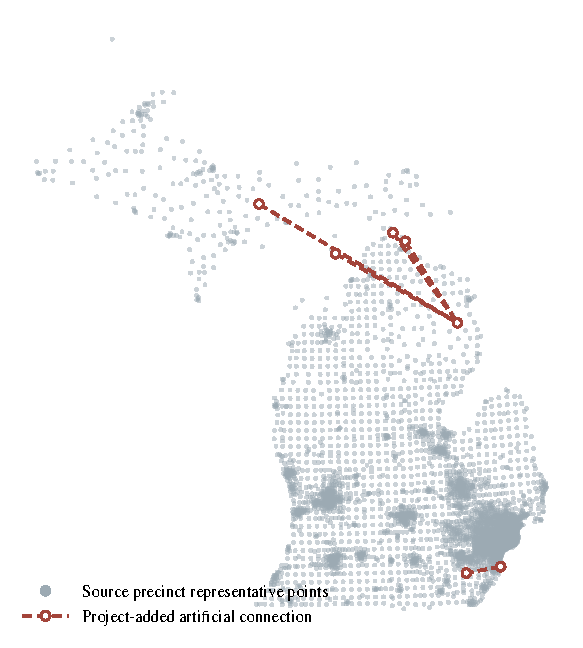
\includegraphics[width=0.91\linewidth]{figures/figure_topology_artificial_bridges.pdf}
\caption{Source-grounded visualization of the five artificial connections inserted by the original project's enacted-label-conditioned graph repair. Faint points are representative locations of the 4,756 Michigan precinct polygons; dashed segments join the closest points on the actual paired polygons. The five source-measured shortest polygon gaps are 42.3, 117.3, 134.3, 169.7 and 280.2 km. Source JSON and polygon ZIP bytes were pinned and independently verified; these lines are not legal land or water routes.}
\label{fig:stage4-1}
\end{figure}

\hypertarget{pillar-ii-the-mixing-illusion}{%
\section{Pillar II: The mixing
illusion}\label{pillar-ii-the-mixing-illusion}}

\hypertarget{original-archived-recom-histories}{%
\subsection{Original archived ReCom
histories}\label{original-archived-recom-histories}}

The earlier Michigan experiment produced long ReCom traces and summary
percentiles. Subsequent audits recovered the original checked-in
research ZIP and independently recomputed 12 complete scalar-metric
histories: six 7,000-state runs under 2016 or 2020 presidential overlays
with nominal ±2\% population tolerance, and six 3,000-state runs under
±1\% or ±3\% tolerances. After the archived burn-in convention, the 2020
±2\% case contained 18,900 correlated recorded states, with mean
Democratic seats 5.7149 and mean efficiency gap −0.0999. The enacted
reference's inclusive Democratic seat-count upper-tail frequency was
2,633/18,900 (13.93\%), while a midrank percentile counted tied values
differently. Such differences are not statistical-significance
estimates: the observations are serially correlated, the target
distribution was not shown to be the legally relevant one, and the
original RNG settings did not make those historic trajectories
replayable from their nominal seed numbers.

The original ±2\% chains also do not satisfy the later, stricter ±0.5\%
population modeling assumption. Among the 18,900 post-burn-in states in
that historical condition, zero met the ±0.5\% tolerance. A sample
cannot be retroactively relabeled as drawn from a more restrictive
feasible space merely because its partisan metrics were calculated
correctly.

\hypertarget{explicit-seed-recom-and-diagnostic-failure}{%
\subsection{Explicit-seed ReCom and diagnostic
failure}\label{explicit-seed-recom-and-diagnostic-failure}}

After correcting GerryChain 1.0's independent random-number generator
initialization, a separate experiment used four dispersed warm starts
under each of two exploratory geographic-constraint regimes. Eight
explicitly seeded ReCom chains, each with 4,001 recorded states,
produced 32,008 serially correlated observations and 648 independently
verified saved assignments. For the efficiency gap, the closer condition
yielded rank-normalized R-hat 1.733 and bulk effective sample size 9.4;
the relaxed condition yielded R-hat 1.139 and bulk ESS 20.4. Both
violated the study's prespecified scalar diagnostics of R-hat no greater
than 1.01 and ESS at least 400.

R-hat and ESS are diagnostics, not proofs of equilibrium; nevertheless,
values this far outside prespecified acceptance criteria are affirmative
grounds not to interpret pooled values as stationary estimates. As
emphasized by Vehtari et al.~(2021), convergence analysis must attend to
inter-chain behavior and autocorrelation rather than the sheer volume of
saved draws. Here, chains often moved noticeably through geographic
space, yet movement did not produce satisfactory mixing on partisan
outcomes.

\hypertarget{reversibility-without-usable-exploration}{%
\subsection{Reversibility without usable
exploration}\label{reversibility-without-usable-exploration}}

The transition law can be known while the explored distribution remains
unreliable. To distinguish an unidentified ReCom transition target from
an interpretable stationary construction, we implemented a local
boundary-edge Metropolis--Hastings (MH) kernel. At state \(x\), the
kernel selects a district-boundary edge, proposes either an oriented
one-precinct transfer or an adjacent two-precinct label swap, and checks
population tolerance, augmented-graph contiguity and fragmentation caps.
Feasible proposals are accepted with
\(\alpha(x,y)=\min\{1,q(y,x)/q(x,y)\}\); failed constraints and rejected
MH proposals are retained as explicit holding self-loops. The proposal
probabilities include the multiplicity with which an assignment change
can arise from choosing different boundary edges. Exact feasible-state
enumeration on a small graph independently verified detailed balance for
the implemented local rule. Consequently, the uniform distribution is
invariant within each reachable communicating component of the labeled,
proxy-feasible assignment space. Nothing in that calculation establishes
that all legal or proxy-feasible maps communicate, or that a finite run
has approached this invariant law.

Why proposals failed in practice. The first source-pinned Michigan MH
pilot generated 2,000 proposals per chain and accepted only
9.20\%--15.95\% across four tested runs. The rejection ledger provides a
more informative diagnosis than acceptance alone. In one closer-cap run,
of 2,000 proposed transitions, 635 failed population checks, 602 failed
contiguity, 547 violated geographic-proxy caps, and 32 were declined by
the MH acceptance correction; just 184 were accepted. These categories
are outcomes of the implemented sequential validation process, not a
factorial estimate of the separate effect of each rule. Tightly balanced
districts make individual precinct transfers difficult; preserving
district connectivity eliminates other local changes; and limited
cut-edge, county and county-subdivision budgets reject additional
otherwise possible candidates. At most, passing all these filters
permits a \emph{local} change. The constrained proposal geometry thus
supplies a concrete mechanism for substantial holding behavior without
proving that the overall state space is disconnected.

Movement and statistical information are different quantities. After
2,000 attempted MH transitions, the four pilot chains changed only
1.7\%--3.7\% of precinct assignments relative to their independently
generated warm starts. In the subsequently executed eight-chain,
4,001-recorded-state study, the efficiency-gap diagnostics remained far
from the prespecified R-hat ≤1.01 and bulk ESS ≥400 gates. The closer
regime produced R-hat 1.568 and bulk ESS 7.1; the relaxed regime
produced R-hat 2.588 and bulk ESS 4.8. The pilot acceptance rates and
later R-hat/ESS figures belong to separate experiments and are not
interchangeable measurements from one chain. Notably, higher local
acceptance under relaxed caps did not yield adequate exploration of the
partisan-score distribution: more accepted transitions do not
necessarily cross the slow modes relevant to the estimand.

The relationship to reversible recombination is a contrast, not a
refutation. Cannon et al.~(2026) establish mathematical reversibility
for a specified spanning-tree-weighted recombination construction; our
local flip/swap MH kernel instead has a uniform invariant law on each
accessible labeled component. The theorems and target distributions
should not be conflated. We separately tested a GerryChain
implementation of a published reversible ReCom variant under two
restrictive pilot configurations; neither 200-proposal pilot changed its
starting assignment. That finite-horizon negative result cannot
establish that the published reversible construction is generally
immobile. It does reinforce the necessity of measuring actual transition
mobility under the \emph{particular} graph, constraints and
implementation in use. The caps tested here are researcher-defined
administrative proxies, not demonstrated to be Michigan's legally
operative districting constraints.

The methodological implication is sharper than a generic injunction to
run longer chains: detailed balance addresses stationarity, whereas
reproducible movement, irreducibility and mixing address whether a
finite research budget can extract information about that law. The
project verified the former within a restricted local model and failed
to demonstrate the latter in its tested Michigan configurations. A
rigorous ensemble report should make this distinction explicit rather
than convert a mathematically plausible transition operator into
unsupported substantive map percentiles.

\hypertarget{pillar-iii-finite-horizon-constraint-stress-testing}{%
\section{Pillar III: Finite-horizon constraint stress
testing}\label{pillar-iii-finite-horizon-constraint-stress-testing}}

\hypertarget{defining-a-finite-horizon-stress-test-estimand}{%
\subsection{Defining a finite-horizon stress-test
estimand}\label{defining-a-finite-horizon-stress-test-estimand}}

Because the neutral stationary target was not verified, the final
experiment deliberately changed the research question. Let \(x_0\) be
the enacted reference assignment and \(P_c\) the implemented stochastic
transition procedure under geographic condition \(c\). Rather than
assert that \(x_T\) approximates a uniform or spanning-tree-weighted
legal map, define the finite-horizon outcome law

\begin{equation}
Q_{c,T}(A)
=\Pr\bigl(X_T\in A\mid X_0=x_{\mathrm{enacted}},
G=G_{\mathrm{KNN3}},P=P_c\bigr),\quad T=800.
\end{equation}

Here \(T=800\) recorded transitions after step zero. The estimand
\(\mathbb{E}_{Q_{c,T}}[f(X_T)]\) is meaningful by construction: it
describes what this particular algorithm produces after a fixed
computational horizon starting from a particular map. It does not imply
a unique stationary target, unbiased representation of legal maps, or
independence of the final state from the enacted reference. This weaker
estimand is the subject of our finite-horizon comparison.

\hypertarget{experiment-protocol}{%
\subsection{Experiment protocol}\label{experiment-protocol}}

We used the source-reconciled KNN3 model graph, an ideal-population
deviation tolerance of ±0.5\%, and GerryChain 1.0 ReCom transitions with
an explicitly initialized, chain-owned RNG. Each run recorded 801 states
including the initial enacted plan. Only its \emph{terminal} state was
retained as a Monte Carlo observation.

Two geographically constrained regimes were examined. The closer regime
permitted at most 760 cut edges, 18 split source county groups, and 20
split source county-plus-MCD groups. The relaxed regime increased these
thresholds to 850, 24, and 49, respectively. The counts are exploratory
proxies, not Michigan statutory compliance determinations. They were
selected in a broader development process involving source and pilot
inspection; the final 64-run protocol fixed them before the final
independent-endpoint results were aggregated, but this is not an
untouched confirmatory preregistration.

For each condition, independently initialized RNG seeds 10001--10032
generated 32 trajectories, producing 64 terminal maps in total. The same
seed labels were used across conditions for bookkeeping; they do not
make the alternative Markov kernels identical. Seed 10001 was replayed
in a separate process in both regimes, reproducing terminal assignment
hashes and complete reported metrics. Each terminal assignment was
independently rescored for 2020 presidential seat counts and efficiency
gap, population equality, proxy fragmentation, source-graph contiguity
and its SHA-256. Both regimes had 32 distinct final assignment hashes.

Sampling \emph{one terminal map per independently seeded run}, rather
than all 51,264 correlated recorded states, makes the Monte Carlo unit
explicit. It does not remove every concern about pseudorandomness or
parameter choice, and 32 terminal maps per condition remain a modest
sample. But it avoids mistaking closely related successive MCMC states
for independent observations when estimating uncertainty about the
finite-time algorithmic mean.

\hypertarget{uncertainty-calculations}{%
\subsection{Uncertainty calculations}\label{uncertainty-calculations}}

For a statistic \(f\), the mean of 32 independent-seed endpoints
estimates \texttt{E\_\{Q\_c,T\}{[}f{]}} under the generator and its
fixed starting map. We used 10,000 nonparametric, deterministic-seed
bootstrap resamples of the 32 endpoints, taking the 2.5th and 97.5th
percentiles to form approximate 95\% Monte Carlo intervals for that
conditional mean. These intervals represent variability among
independent runs of this algorithm, not uncertainty about a legally
neutral map distribution or a claim of generalizing to other election
years.

For the descriptive indicator that an endpoint's efficiency gap is at
least the enacted reference efficiency gap, we computed the observed
proportion and Wilson 95\% binomial interval. Since the enacted map is
also the deterministic starting state, and the model and caps are
researcher-designed, the resulting fraction must not be described as an
enacted-map randomization p-value.

\hypertarget{results-quantifying-the-constraint-shift}{%
\section{Results: Quantifying the constraint
shift}\label{results-quantifying-the-constraint-shift}}

\hypertarget{terminal-partisan-scores-and-geographic-movement}{%
\subsection{Terminal partisan scores and geographic
movement}\label{terminal-partisan-scores-and-geographic-movement}}

\begin{table}[H]
\centering
\caption{Terminal outcomes after 800 recorded transitions under two exploratory geographic regimes.}
\label{tab:endpoints}
\begin{threeparttable}
\footnotesize
\begin{tabularx}{\linewidth}{@{}>{\raggedright\arraybackslash}X
>{\raggedleft\arraybackslash}p{0.287\linewidth}
>{\raggedleft\arraybackslash}p{0.287\linewidth}@{}}
\toprule
Outcome & Tighter constraints & Relaxed constraints\\
\midrule
Democratic seats & 7.219 [7.000, 7.438] & 6.813 [6.594, 7.031]\\
Efficiency gap & +0.02010 [+0.00300, +0.03722] &
$-0.01268$ [$-0.03036$, +0.00458]\\
Cut edges, KNN3 graph & 695.09 [686.00, 703.75] & 758.84 [746.66, 771.16]\\
Split source county groups & 17.97 [17.91, 18.00] & 23.81 [23.63, 23.97]\\
Split county--MCD groups & 19.94 [19.84, 20.00] & 47.94 [47.50, 48.34]\\
Reassigned precincts (\%) & 13.40 [12.05, 14.81] & 29.00 [27.75, 30.29]\\
\bottomrule
\end{tabularx}
\begin{tablenotes}[flushleft]
\footnotesize
\item \emph{Note.} Means and 95\% percentile bootstrap intervals from 32 independently seeded
terminal maps per condition. The 2020 presidential-vote overlay is counterfactual.
The proximity graph and fragmentation caps are not certified as Michigan legal rules.
\end{tablenotes}
\end{threeparttable}
\end{table}

Figures 2--4 present empirical terminal outcomes from the 64
independently verified endpoint maps. Together, they show how the
constraint regimes affect the efficiency-gap distribution, the
correspondence between seed-indexed runs, and spatial movement from the
enacted reference.

\begin{figure}[H]
\centering
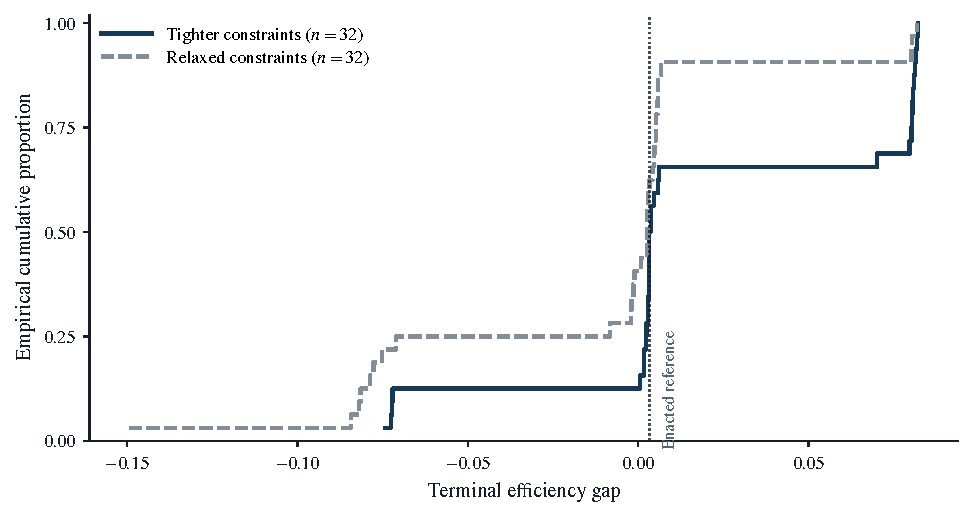
\includegraphics[width=0.90\linewidth]{figures/figure1_terminal_EG_ECDF.pdf}
\caption{Empirical cumulative distributions of efficiency gap under tighter and relaxed model constraints (32 independently seeded endpoints per regime). The vertical reference marker is the enacted plan under the same 2020 presidential-vote overlay; this is not a legal-map outlier test.}
\label{fig:stage4-2}
\end{figure}

\begin{figure}[H]
\centering
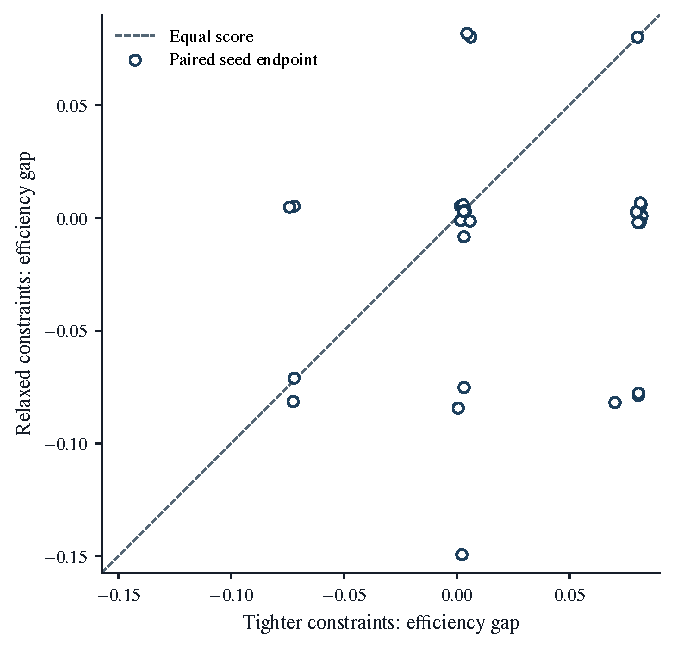
\includegraphics[width=0.71\linewidth]{figures/figure2_paired_seed_EG.pdf}
\caption{Efficiency-gap scores by shared seed identifier across the two regimes. The dashed diagonal marks equal values. Shared seed numbers do not imply identical proposals or matched geographic plans.}
\label{fig:stage4-3}
\end{figure}

\begin{figure}[H]
\centering
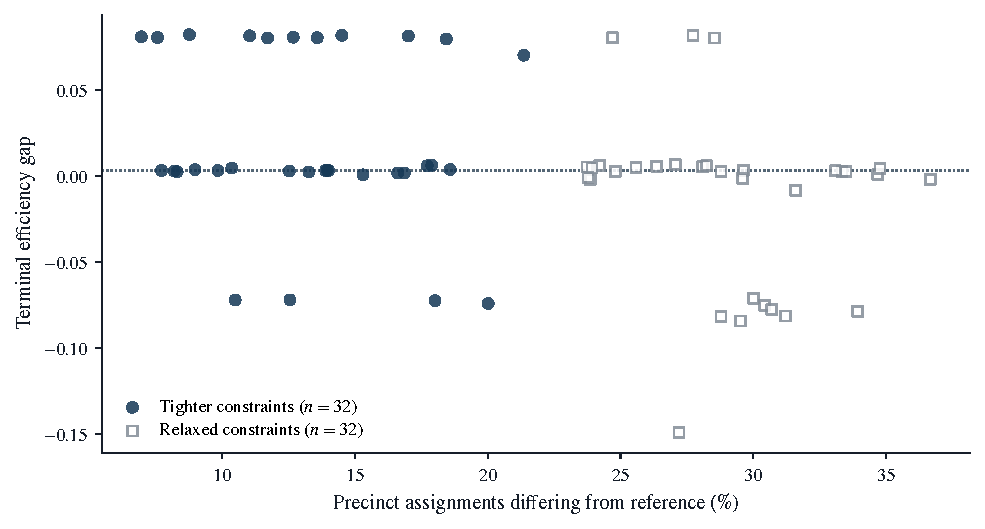
\includegraphics[width=0.90\linewidth]{figures/figure3_spatial_change_vs_EG.pdf}
\caption{Endpoint efficiency gap versus the fraction of precincts reassigned from the enacted reference after optimal label matching. Candidate geography is defined by the experimental proximity graph.}
\label{fig:stage4-4}
\end{figure}

Detailed data fingerprints, source-checked plotting code, and
figure-generation logs are supplied in the reproducibility appendix.

The tighter model produces terminal plans closer to the original
geography by every reported fragmentation measure and yields modestly
higher Democratic seat scores under the selected election layer. Mean
efficiency gaps differ by about 0.0328 (3.28 percentage points of the
efficiency-gap scale) between regimes, while mean Democratic seats
differ by about 0.406 seats. These are differences between specified
finite-time algorithmic procedures, not a causal estimate of how legally
valid district maps would respond to relaxing real Michigan law.

The geometry contrast is particularly strong. Under the closer regime,
an endpoint differs from the enacted assignment at approximately 13.4\%
of precinct nodes after optimal district-label matching; under the
relaxed regime, 29.0\%. The chains also reject a large share of
attempted geographic proposals: on average 79.22\% under closer caps and
52.83\% under relaxed caps. Lower geometric movement under tighter caps
is consistent with more severe constraints on feasible proposals.
However, the rejected-proposal rate is an implementation diagnostic and
does not prove any particular legal or political mechanism.

Read together, Table 1, Figure 4 and the paired-seed contrast in Table 2
provide a concrete account of the tested algorithmic sensitivity. Mean
distance from the enacted assignment increases from 13.40\% to 29.00\%
of precinct nodes under optimal relabeling, while the relaxed regime
also has 63.75 more cut edges on average. Over the same change in
composite cap regime, mean Democratic seats decrease by 0.406 and mean
efficiency gap decreases by 0.03278. Thus increased feasible
fragmentation, increased terminal geographic movement and a signed
partisan-score shift co-occur within the fixed 800-transition procedure.
Figure 4 visualizes movement and efficiency gap for individual
endpoints; Table 2 quantifies a mean regime contrast. Neither
establishes that geographic movement mediates the partisan change or
that any one administrative cap is the causal driver.

The closer condition concentrates near its caps on county and
county-plus-MCD splits (means 17.97 of 18 and 19.94 of 20). The relaxed
condition approaches its much larger bounds (means 23.81 of 24 and 47.94
of 49). Because the baseline itself has only 14 split source county
groups and 9 split county-plus-MCD groups, both models can diverge
materially from the reference's administrative fragmentation. A headline
suggesting ``maps just like the enacted one except for partisan
choices'' would therefore misdescribe the sample-generating assumptions.

\hypertarget{enacted-reference-frequencies-under-the-tested-procedure}{%
\subsection{Enacted-reference frequencies under the tested
procedure}\label{enacted-reference-frequencies-under-the-tested-procedure}}

The 2020-reference efficiency gap is about +0.00333. In the closer
regime, 16 of 32 terminal simulated gaps were at least that value
(50.0\%; Wilson 95\% interval approximately 33.6--66.4\%). In the
relaxed regime, 13 of 32 met the same criterion (40.6\%; Wilson interval
approximately 25.5--57.7\%). Neither fraction provides a legal-map null
probability. The generator is initialized \emph{at} the enacted
reference, the model topology is a geometry-proximity approximation, and
the two cap regimes are researcher-selected. Consequently, no inference
about intent, statutory validity or statewide partisan extremeness
follows from these percentages.

The findings support a different, narrower statement: within 800
recorded ReCom transitions from the same reference and on the same
experimental proximity graph, choices about fragmentation caps were
associated with materially different geographic movement and
distributions of partisan scores. The experiment makes that conditional
relationship observable and reproducible. It does not identify which cap
choice is socially, legally or scientifically neutral.

\hypertarget{signed-paired-seed-contrasts}{%
\subsection{Signed paired-seed
contrasts}\label{signed-paired-seed-contrasts}}

Because each cap regime was run under the same 32 nominal pseudorandom
seeds, one can report differences between the corresponding terminal
outcomes indexed by seed, rather than relying solely on two separate
sets of condition means.

The paired endpoint contrast for any reported statistic \(f\) is

\begin{equation}
\widehat{\Delta}_f
=\frac{1}{32}\sum_{s=10001}^{10032}
\left[
f\!\left(X_{800,s}^{\mathrm{tight}}\right)
-f\!\left(X_{800,s}^{\mathrm{relaxed}}\right)
\right].
\end{equation}

We retained the paired indexing of the original fixed-horizon experiment
and drew 20,000 bootstrap resamples of entire seed-indexed endpoint
pairs, not individual correlated chain steps. A deterministic resampling
seed (20261018) makes the interval calculation reproducible.

\begin{table}[H]
\centering
\caption{Paired-seed terminal contrasts: tighter minus relaxed conditions.}
\label{tab:paired}
\begin{threeparttable}
\footnotesize
\begin{tabularx}{\linewidth}{@{}>{\raggedright\arraybackslash}X
>{\raggedleft\arraybackslash}p{0.18\linewidth}
>{\raggedleft\arraybackslash}p{0.31\linewidth}@{}}
\toprule
Terminal outcome & Mean difference & 95\% bootstrap interval\\
\midrule
Democratic seats & +0.406 & [+0.124, +0.719]\\
Efficiency gap & +0.03278 & [+0.00975, +0.05631]\\
KNN3 cut edges & $-63.75$ & [$-80.06$, $-46.91$]\\
Reassigned precincts (pp) & $-15.61$ & [$-17.79$, $-13.50$]\\
\bottomrule
\end{tabularx}
\begin{tablenotes}[flushleft]
\footnotesize
\item \emph{Note.} 32 seed-indexed pairs; 20,000 bootstrap resamples.
pp denotes percentage points. The regimes alter several caps simultaneously.
The contrasts are neither legal-map neutrality tests nor isolated causal effects.
\end{tablenotes}
\end{threeparttable}
\end{table}

The paired bootstrap uses the joint seed-indexed output of the two
programs. Its precision is conditional on the fixed, researcher-selected
comparison and approximate independence across the 32 separate RNG seed
labels. It does not imply identical stochastic proposals within a pair,
actual matched districts, or isolation of any one cap, because the
cut-edge, county-split and MCD-split caps changed simultaneously. The
results nonetheless sharpen the descriptive finding: the two
finite-horizon procedures have distinguishable outcomes in this executed
computational experiment. They supply no additional evidence that either
procedure samples neutral, legally valid Michigan plans.

\hypertarget{baseline-reliability-a-three-gate-evidentiary-protocol}{%
\section{Baseline reliability: A three-gate evidentiary
protocol}\label{baseline-reliability-a-three-gate-evidentiary-protocol}}

A recommendation to ``validate the simulation'' provides little guidance
about which failures must stop a substantive claim. We instead propose
three operational gates. Each identifies required evidence, a failure
condition, and the disposition of the Michigan case. This is an
auditable reporting and stress-testing procedure, not a newly proven
statistical test.

\hypertarget{gate-a-validate-topology-independently-of-the-enacted-map}{%
\subsection{Gate A --- Validate topology independently of the enacted
map}\label{gate-a-validate-topology-independently-of-the-enacted-map}}

Required evidence. Archive input polygon and election provenance, graph
construction rules, an explicit list of synthetic adjacencies, and
geographic distances or statutory island connections for exceptional
edges. Test the enacted reference's connectivity only after choosing
edges without using its district labels.

Failure condition. Connectivity is created through
enacted-label-dependent links, or invented adjacency is treated as
physical/legal contact without supporting evidence.

Case decision. The original five enacted-conditioned artificial edges
linked precinct polygons approximately 42--280 km apart. A
district-blind KNN3 alternative adds 13 candidate links, with maximum
polygon separation 17.8 km, while retaining reference connectivity.
However, KNN3 was selected after reference-compatibility testing and
remains legally uncertified. Source geometry matching passed; legal
geography did not pass this gate.

\hypertarget{gate-b-verify-the-claimed-sampling-law-and-substantive-mixing}{%
\subsection{Gate B --- Verify the claimed sampling law and substantive
mixing}\label{gate-b-verify-the-claimed-sampling-law-and-substantive-mixing}}

Required evidence. Specify the target law or explicitly state that the
result estimates a finite-horizon procedure. For stationary ensemble
claims, evaluate multiple appropriate starting maps, proposal/holding
behavior, assignment mobility, rank-normalized R-hat, and bulk/tail
effective sample size for substantive partisan metrics. Publish the
acceptance criteria and actual failures.

Failure condition. The law is unidentified, the diagnostic plan is
missing, or the chain fails its declared convergence criteria. Saving
more highly correlated maps is not a substitute for meeting these
conditions.

Case decision. Eight-chain studies recorded 32,008 states and
independently checked 648 full assignments, but the tested ReCom and
local MH configurations failed their prespecified thresholds (R-hat
≤1.01, bulk and tail ESS ≥400). For efficiency gap, ordinary ReCom gave
R-hat 1.733 with bulk ESS 9.4 in one condition; local MH yielded R-hat
2.588 with ESS 4.8 in another. These experiments do not establish a
usable stationary neutral ensemble. They do not imply a universal
failure of all redistricting samplers.

Theoretical guarantee versus operational mobility. DeFord, Duchin, and
Solomon (2021) motivate recombination moves, while Cannon et al.~(2026)
establish reversibility for a particular spanning-tree-targeting
construction. Our reversible local MH implementation instead targets a
uniform distribution within each reachable component of a proxy-feasible
labeled-map space. In its initial four-chain pilot, acceptance ranged
from 9.20\% to 15.95\% after 2,000 proposals per chain; in the
subsequent eight-chain study, acceptance varied from 8.20\% to 16.75\%,
while the relaxed-regime efficiency-gap diagnostic reached R-hat 2.588
and bulk ESS about 4.8 after 4,001 recorded states per chain. The
acceptance and convergence figures come from different runs, and neither
evaluates Cannon et al.'s spanning-tree kernel directly. Their joint
methodological lesson is narrower and stronger than a claim that
mathematics failed: detailed balance need not imply adequate mobility or
finite-time convergence under restrictive geographic proxies.

\hypertarget{gate-c-quantify-sensitivity-to-declared-constraint-alternatives}{%
\subsection{Gate C --- Quantify sensitivity to declared constraint
alternatives}\label{gate-c-quantify-sensitivity-to-declared-constraint-alternatives}}

Required evidence. Define credible alternative rules, hold the remaining
experimental setup fixed where possible, measure signed changes in the
outcome of interest, and estimate uncertainty from appropriate
independent units. Explain when several constraints change at once.

Sensitivity flag. An estimated procedure contrast whose uncertainty
interval excludes zero identifies a detected difference at the tested
horizon and computational precision. This is a model-choice warning, not
a legal decision rule or a test that an enacted map was manipulated.

Case decision. Relative to tighter caps, relaxed \emph{composite} caps
produced 15.61 percentage points more precinct reassignment, 0.406 fewer
Democratic seats, and 0.03278 lower efficiency gap under the fixed
overlay. The tighter-minus-relaxed efficiency-gap 95\% paired bootstrap
interval is {[}+0.00975, +0.05631{]}. Since cut-edge, county-split, and
county--MCD caps changed jointly, the individual effect of any one rule
is not identified.

\hypertarget{operational-evidence-checks-tied-to-executable-artifacts}{%
\subsection{Operational evidence: checks tied to executable
artifacts}\label{operational-evidence-checks-tied-to-executable-artifacts}}

The protocol is more useful when every claim resolves to a specific test
rather than a blanket statement that the repository has continuous
integration. Source integrity is implemented through
\texttt{download\_source.py}, \texttt{verify\_graph.py}, and
\texttt{docs/data\_provenance.md}: they pin the upstream Michigan JSON
and polygon ZIP and reconcile all 4,756 processed precinct records. This
is processed-data provenance; the original Census/VEST precinct joins
have not been independently rerun. The graph and polygon identities are
part of the audit input, not substitutes for legal-island or Voting
Rights Act verification.

Topological evidence is retained by \texttt{stage3-bridge-audit.yml},
\texttt{stage3-geometric-mst-candidates.yml}, and
\texttt{stage3-topology-gate.yml}. These checks distinguish the original
long-range, enacted-conditioned bridges from distance-minimizing
component connectors and the KNN3 sensitivity graph. Their scientific
verdicts are interpreted from the generated audit outputs, not inferred
from a green workflow icon. Indeed, the original component-level
minimum-spanning-tree proposal does \emph{not} make every enacted
reference district connected, despite being obtained from an
independently specified spatial-distance objective.

Mathematical evidence is maintained in
\texttt{stage2\_mathematical\_validation.md}. Independent recomputation
established the seat and efficiency-gap sign conventions and isolated a
one-vote-level 2016 threshold discrepancy arising from fractional
precinct-vote allocations and floating-point summation order. The lesson
is not that the efficiency gap is inherently unreliable; it is that a
partisan metric's implementation, threshold rules, and numerical
tolerances should be independently reconciled before inference. Sampling
evidence includes the later MH pilots, acceptance/rejection counters,
and explicit warm-start assignment distances. The four-condition MH
pilot accepted approximately 9.20\%--15.95\% of proposals and moved only
1.7\%--3.7\% of precinct assignments from warm starts after 2,000
attempts; subsequent eight-chain diagnostics failed. A separate
GerryChain 1.0 RNG erratum documents how Python-global seeding failed to
initialize the library-owned chain generator. It justifies a
version-specific reproducibility fix in this project, not an assertion
that other published studies are unreplayable.

Configuration as an executed research protocol. In simulation-based
inference, publishing source code is necessary but insufficient: a
reader must know which code paths, graph files, parameters and RNG
streams generated the \emph{reported} sample rather than some other
possible run of the same repository. The
\texttt{stage3-finite-horizon-ensemble.yml} workflow records the final
eight-job matrix covering the 32 seeds per model regime (10001--10032),
exact cap triples (760, 18, 20) and (850, 24, 49), 801 recorded states
per trajectory, and the ±0.5\% district-population tolerance. The matrix
passes the settings to executable command-line arguments; the generator
rejects inconsistent condition/cap combinations; the aggregation refuses
missing and duplicated seed identities, graph-digest disagreements,
incorrect horizon metadata, and independently rescored invalid terminal
maps. The workflow also retains dependency inventories and separately
replays seed 10001 in each condition to check complete endpoint records.
These measures make the \emph{executed} configuration inspectable, not
simply imaginable from an unused template.

Cryptographic fingerprints and the provenance chain. The upstream
processed Michigan graph and polygon ZIP are identified by pinned Git
blob SHA-1s, and the generated KNN3 sensitivity graph has SHA-256 digest
\texttt{\seqsplit{14355742f58291f4c26267982de07a21037c347f7598a68f032e0d68ea1d542c}}.
Recorded seeds, terminal-assignment SHA-256 hashes and
source-independent terminal rescoring link each retained observation to
its modeled inputs. For final figures, the Stage 4 plotting workflow
retrieves the specific successful 64-endpoint result artifact, checks
its provenance and endpoint identities, and generates the efficiency-gap
and movement graphics by code rather than manual spreadsheet
rearrangement. The earlier
\texttt{outputs/figures/week1/mi\_week1\_summary\_dashboard.png}
illustrates automated descriptive reporting at the project's initial
stage; it is not the evidentiary source of the later 64-endpoint
estimates. This traceable sequence limits unrecorded intervention
between scoring and presentation, while still allowing a reviewer to
inspect what every transformation does.

What the fingerprints cannot prove. A cryptographic checksum confirms
equality to specified bytes when checked, not that the bytes encode
appropriate legal geography, valid source joins or an unbiased analysis.
The original upstream Census/VEST joins were not independently
reconstructed; a mutable repository branch is not an immutable signed
research archive; and dependency inventories do not constitute complete
container-image pinning. Researchers deliberately selected the model
graph, parameters and stopping horizon during exploratory development.
The final matrix makes the executed comparison reproducible, but it does
not erase that researcher discretion or convert the study into an
externally preregistered experiment. This is a positive methodological
finding: provenance tests make hidden choices \emph{detectable and
discussable}, not nonexistent.

Toward an adversarial computational evidence ledger. We propose that
simulation-based redistricting research release not only a successful
result but a machine-checkable record of what can cause the result to be
rejected: (1) exact input and derived-graph identifiers; (2) tests that
intentionally supply impossible district assignments, invalid population
deviations, corrupt or nonfinite vote fields, and malformed state
sequences; (3) RNG initialization and cross-process replay tests; (4)
independent validity and scoring checks for the archived assignments;
and (5) prespecified diagnostic and assumption-sensitivity gates with
failed outcomes preserved. The current
\texttt{stage12-reproducibility.yml} and
\texttt{stage4-manuscript-validation.yml} workflows support different
components of this ledger. In the reported 64-run experiment, all 64
retained terminal maps were independently rescored and verified; in the
longer MCMC pilots, a selection of periodic full assignments was
independently checked. That evidence is not equivalent to independently
checking every intermediate MCMC map, although the generator applies its
own run-time constraints. The known one-vote-level 2016 score
discrepancy and corrected GerryChain RNG initialization illustrate why
adversarial numerical and reproducibility checks matter even when
ordinary execution succeeds.

Implications for research and expert evidence. The evidentiary demand
should be proportional to the conclusion. A histogram described merely
as the behavior of a fixed finite-horizon algorithm may require exact
procedural reconstruction; a histogram offered as a neutral distribution
over \emph{legally permissible plans} additionally demands independently
defensible adjacency, legal constraints, target law and credible mixing
diagnostics. We therefore recommend that journals, external reviewers
and courts evaluating such testimony request inspectable computational
audit ledgers and decline to treat undocumented ensemble percentiles as
self-validating. This is a proposed scientific reporting standard, not a
claim that the repository can determine legal admissibility or certify
compliance with Michigan law.

The Stage 4 pipeline then downloads the specific successful 64-endpoint
artifact, refuses a mismatched graph digest, duplicate endpoint hash or
missing seed, recalculates paired contrasts, and generates vector
figures and genuine XeLaTeX. Its programmatic output is an automated,
source-linked research artifact, not a substitute for independently
checking GIS topology, the interpretation of statistics, or the code
that constructs each visualization.

\begin{table}[H]
\centering
\caption{Executable evidence and scientific disposition of baseline reliability checks.}
\label{tab:audit-gates}
\begin{threeparttable}
\footnotesize
\begin{tabularx}{\linewidth}{@{}>{\raggedright\arraybackslash}p{.21\linewidth}
>{\raggedright\arraybackslash}p{.33\linewidth}
>{\raggedright\arraybackslash}X@{}}
\toprule
\textbf{Audit layer} & \textbf{Inspectible records} & \textbf{Scientific disposition}\\
\midrule
Source geography & Exact graph and polygon digests; artificial-bridge audit; component-MST and KNN3 tests
& Processed inputs reconciled; authoritative legal adjacency unresolved\\
Numerical definitions & Independent seat, population, compactness, efficiency-gap calculations
& Arithmetic reconciles; 2016 one-vote threshold-order difference disclosed\\
Sampling reliability & Corrected RNG replay; warmup distances; rejection logs; rank R-hat and bulk/tail ESS
& Tested stationary-null diagnostics fail\\
Constraint sensitivity & Versioned 64-run workflow, individually verified terminal maps, paired contrast uncertainty
& Signed finite-horizon procedure difference detected; individual cap effect not identified\\
Paper reproducibility & Graph and endpoint SHA gates; programmatic vector plots; XeLaTeX/visual PDF checks
& Source-linked document verified; not external scientific review\\
\bottomrule
\end{tabularx}
\begin{tablenotes}[flushleft]
\footnotesize
\item \emph{Note.} Source, numerical, or build success is not itself certification of a legal neutral-map distribution.
\end{tablenotes}
\end{threeparttable}
\end{table}

\hypertarget{the-evidentiary-consequence}{%
\subsection{The evidentiary
consequence}\label{the-evidentiary-consequence}}

The three gates perform distinct jobs: topology determines which
district plans are representable; sampling evidence determines whether
output supports a specified probability law; and sensitivity analysis
measures dependence on defensible assumptions. Passing one does not
compensate for failing another.

For the present case, numerical execution is reproducible and the
finite-horizon constraint sensitivity is quantifiable. A statewide legal
neutral-map null has not passed the necessary topology and convergence
conditions. This supports an actionable principle for methodological
research and evaluation of expert evidence: a simulation-based baseline
should be accompanied by independently verifiable graph provenance,
target-law/mixing records, and model-choice sensitivity results before
its percentiles are assigned substantive authority.

The preliminary
\href{https://github.com/DjokovicMan22/Gerrymandering-Project/blob/research/stages-1-3-validation/outputs/figures/week1/mo_precinct_dual_graph_overlay.png}{Missouri
precinct graph overlay} and related graphics are descriptive outputs of
earlier exploratory work; Missouri's historic local inputs were not
byte-matched to the candidate published Missouri source, and a matched
independent graph-component and ensemble audit has not been performed.
These plots cannot be used as a second-state replication. We have not
audited a representative sample of published studies or courtroom
testimony. The broader prevalence of such failures remains a testable
question for subsequent research, not a result of this Michigan case.

\hypertarget{scope-of-the-audit-and-boundaries-of-inference}{%
\section{Scope of the Audit and Boundaries of
Inference}\label{scope-of-the-audit-and-boundaries-of-inference}}

The first and largest limitation is legal and geographic. The repaired
KNN3 graph is an experimentally chosen proximity approximation, not a
certified Michigan island, shoreline, municipal, Voting Rights Act or
communities-of-interest model. The absence of detailed VRA and community
constraints precludes legal plan probability claims. In addition, the
source polygons and election allocations are processed public
derivatives; the original raw Census/VEST joining pipeline and agreement
with official election canvasses have not been fully rebuilt.

Second, the election overlays are historically displaced: 2016 and 2020
presidential returns are allocated to a plan adopted in 2021. They do
not account for candidate-specific congressional voting, later shifts in
turnout, incumbency or strategic responses to new district lines. Third,
efficiency gap and seat count summarize only selected aspects of
representation; their interpretation depends on turnout, geography,
competitiveness and the aggregation rule.

Fourth, the historic simulation archives do not preserve every precinct
assignment or the correctly initialized chain RNG stream; their original
transitions cannot be independently reconstructed from saved scalar
scores alone. While new tests verify all finite-horizon terminal maps,
the 64-run experiment was not designed to establish stationary
convergence. The two geographic conditions differ in several cap
thresholds simultaneously, so their score difference cannot be
attributed to a single administrative constraint. The sample size of 32
endpoints per condition permits only modest-precision conditional Monte
Carlo summaries. Finally, KNN3 and the constraint regimes emerged
through exploratory development, and the final finite-horizon protocol
was fixed only after that preliminary search; the analysis should not be
presented as an externally preregistered confirmatory test.

These limitations do not contradict the empirical findings. They
determine the scale of claims those findings can support.

\hypertarget{conclusion}{%
\section{Conclusion}\label{conclusion}}

Neutrality cannot be inferred from the size or reproducibility of an
ensemble. Our Michigan experiments document three independent points of
vulnerability: enacted-label-conditioned graph repairs linked polygons
separated by approximately 42--280 km; tested ReCom and local reversible
MH configurations failed prespecified convergence criteria; and a 64-run
finite-horizon stress test detected changes in partisan and spatial
outcomes across two constraint regimes. The tighter-minus-relaxed
efficiency-gap contrast was +0.03278, with a conditional
paired-bootstrap interval {[}+0.00975, +0.05631{]}.

The finding is not merely that permissive caps increase geographic
movement. It is that an apparently precise baseline has three distinct
layers requiring independent justification: the graph that defines
possible maps, the sampler that assigns probability, and the assumptions
that determine what results remain stable. The Michigan case quantifies
concrete failure modes in each layer without claiming a stationary
distribution over legally permissible maps.

Our practical contribution is a three-gate audit with falsifiable
refusal conditions: validate synthetic geography independently,
demonstrate target-specific sampler reliability, and quantify
sensitivity to consequential constraints. These gates motivate an
adversarial computational evidence ledger---versioned executed
parameters, exact input and output identities, corruption-rejection
tests, independent replay, map-validity checks, and transparent records
of statistical failures. Such evidence should be inspectable before a
simulation is invoked as a neutral comparison. The absence of partisan
variables in a transition script is not, by itself, evidence of a
neutral sampling distribution: a benchmark can inherit political or
geographic structure through topology repair, feasibility definitions,
initialization, and researcher-selected thresholds.

For academic evaluation and litigation alike, the appropriate response
is not to presume that computational redistricting is unsound; it is to
require that the \emph{particular inferential bridge} from code to
claimed baseline be demonstrated. A passed CI job means that specified
checks ran successfully, not that the simulated maps satisfy every
geographic or statutory condition. A proof of detailed balance does not
establish finite-budget convergence. A tightly estimated difference
between two finite-horizon procedures does not identify the effect of a
single legal rule. The Michigan evidence exposes each distinction with
an executable failure case and a signed sensitivity result. These
distinctions belong in the evidentiary standard for computational
baselines, not in optional technical footnotes. Determining the
prevalence of comparable weaknesses in published research, other states,
and litigation remains a priority for separate systematic study; the
present experiment demonstrates a concrete methodological vulnerability,
not its national frequency.

\hypertarget{references}{%
\section*{References}\label{references}}
\addcontentsline{toc}{section}{References}

\begingroup\small
\setlength{\parindent}{0pt}
\setlength{\parskip}{5pt}
\begin{hangparas}{1.25em}{1}

Cannon, Sarah, Moon Duchin, Dana Randall, and Parker Rule. 2026. “Spanning Trees and Redistricting: New Methods for Sampling and Validation.” *SIAM Review* 68 (2): 349–381. https://doi.org/10.1137/24M166944X.

Chikina, Maria, Alan Frieze, and Wesley Pegden. 2017. “Assessing Significance in a Markov Chain without Mixing.” *Proceedings of the National Academy of Sciences* 114 (11): 2860–2864. https://doi.org/10.1073/pnas.1617540114.

DeFord, Daryl, Moon Duchin, and Justin Solomon. 2021. “Recombination: A Family of Markov Chains for Redistricting.” *Harvard Data Science Review* 3 (1). https://doi.org/10.1162/99608f92.eb30390f.

Kenny, Christopher T., Cory McCartan, Tyler Simko, Shiro Kuriwaki, and Kosuke Imai. 2023. “Widespread Partisan Gerrymandering Mostly Cancels Nationally, but Reduces Electoral Competition.” *Proceedings of the National Academy of Sciences* 120 (25): e2217322120. https://doi.org/10.1073/pnas.2217322120.

McCartan, Cory, Christopher T. Kenny, Tyler Simko, George Garcia III, Kevin Wang, Melissa Wu, Shiro Kuriwaki, and Kosuke Imai. 2022. “Simulated Redistricting Plans for the Analysis and Evaluation of Redistricting in the United States.” *Scientific Data* 9. https://doi.org/10.1038/s41597-022-01808-2.

Michigan Constitution of 1963, art. IV, § 6(13). Michigan Legislature. https://legislature.mi.gov/Laws/MCL?objectName=mcl-Article-IV-6.

Stephanopoulos, Nicholas O., and Eric M. McGhee. 2015. “Partisan Gerrymandering and the Efficiency Gap.” *University of Chicago Law Review* 82 (2): 831–900. https://chicagounbound.uchicago.edu/uclrev/vol82/iss2/4/.

Vehtari, Aki, Andrew Gelman, Daniel Simpson, Bob Carpenter, and Paul-Christian Bürkner. 2021. “Rank-Normalization, Folding, and Localization: An Improved R-hat for Assessing Convergence of MCMC.” *Bayesian Analysis* 16 (2): 667–718. https://doi.org/10.1214/20-BA1221.

Veomett, Ellen, with Arbie Hsu and Alusi. “Michigan JSON and Shapefile” (processed precinct GIS, election and population data; source README and notebook). Source materials obtained from the Redistricting Data Hub, June 2024. https://github.com/eveomett-states/Michigan. CC BY-NC 4.0 and applicable Redistricting Data Hub conditions.



\end{hangparas}
\endgroup

\clearpage
\appendix

\hypertarget{reproducibility-and-evidence-appendix}{%
\section{Reproducibility and evidence
appendix}\label{reproducibility-and-evidence-appendix}}

A. Processed input fingerprints. Michigan original graph Git blob SHA-1:
\texttt{\seqsplit{a4dfe70818f87b97924781216f3d86a672cfc66a}}. Original
polygon ZIP Git blob SHA-1:
\texttt{\seqsplit{07bce18dabbcca9d549e28995a8156fd6978d7db}}. Derived
KNN3 graph SHA-256:
\texttt{\seqsplit{14355742f58291f4c26267982de07a21037c347f7598a68f032e0d68ea1d542c}}.
Historical archive ZIP SHA-256:
\texttt{\seqsplit{0f52e51f8b64d1f2bc93b2e4fc206f824d777d494a90ae8a278461bac48736d4}}.

B. Exact computational environment. The main experimental dependency is
\texttt{gerrychain==1.0.0} with Python 3.11, networkx, numpy, pandas and
geopandas/shapely. CI captures dependency versions. Both condition
cohorts used deterministic \texttt{PYTHONHASHSEED=0}, independently
seeded chain RNG streams and per-run assignment/graph hashes.

C. Audited original source, geometry and mathematics.
\href{https://github.com/DjokovicMan22/Gerrymandering-Project/blob/research/stages-1-3-validation/docs/research_audit/STAGE12_FINAL_VERIFICATION.md}{Stage
1--2 verification report};
\href{https://github.com/DjokovicMan22/Gerrymandering-Project/actions/runs/39183949679}{successful
independent source, history and compactness CI};
\href{https://github.com/DjokovicMan22/Gerrymandering-Project/blob/research/stages-1-3-validation/docs/data_provenance.md}{source
provenance record}.

D. Nonconvergence and model construction.
\href{https://github.com/DjokovicMan22/Gerrymandering-Project/blob/research/stages-1-3-validation/docs/research_audit/stage3_diversified_sampling_results.md}{Original
diversified ReCom diagnostics};
\href{https://github.com/DjokovicMan22/Gerrymandering-Project/blob/research/stages-1-3-validation/docs/research_audit/stage3_reversible_mixing_results.md}{reversible
local-chain diagnostics};
\href{https://github.com/DjokovicMan22/Gerrymandering-Project/blob/research/stages-1-3-validation/docs/research_audit/stage3_finite_horizon_protocol.md}{geographic
bridge analysis and finite-horizon protocol}.

E. Independently seeded endpoint experiment.
\href{https://github.com/DjokovicMan22/Gerrymandering-Project/actions/runs/39180152601}{Successful
64-run GitHub Actions workflow, derived CSV endpoints, JSON summary and
seed replay evidence};
\href{https://github.com/DjokovicMan22/Gerrymandering-Project/blob/research/stages-1-3-validation/docs/research_audit/STAGE3_FINAL_REPORT.md}{Stage
3 final empirical report}. The published workflow artifact contains
model-specific derived scores but excludes redistributed third-party
source graphs and full precinct assignment maps.

F. Plotting and paired contrasts.
\href{https://github.com/DjokovicMan22/Gerrymandering-Project/actions/runs/39203488689}{Stage
4 source-audited graphics and paired Monte Carlo computation};
production code in
\texttt{scripts/research\_audit/stage4\_journal\_figures.py}. Input is
the original Stage 3 aggregate artifact, strictly checked by SHA and
seed identities. Contrasts concern the researcher-defined finite-horizon
procedures only.

G. Status and interpretation. This is a methods and
conditional-sensitivity manuscript; numerical computations and scoped
reproducibility checks passed, while legal-plan stationarity,
authoritative geographic admissibility and an enacted-map outlier
hypothesis were not established. This manuscript should undergo external
methodological review before submission. The reported conditional
bootstrap intervals and endpoint frequencies are not gerrymandering
significance tests.

\end{document}
